%% LyX 2.0.0 created this file.  For more info, see http://www.lyx.org/.
%% Do not edit unless you really know what you are doing.
\documentclass[12pt,brazil]{article}
\usepackage[T1]{fontenc}
\usepackage[utf8]{inputenc}
\usepackage{amsmath}
\usepackage{amssymb}
\usepackage{graphicx}

\makeatletter

%%%%%%%%%%%%%%%%%%%%%%%%%%%%%% LyX specific LaTeX commands.
%% A simple dot to overcome graphicx limitations
\newcommand{\lyxdot}{.}


\makeatother

\usepackage{babel}
\begin{document}

\title{Aula Exercício de Introdução ao SSH}


\author{Henrique Gemignani Passos Lima}

\maketitle
\tableofcontents{}


\section{O que é SSH, e principais características}

SSH, Secure Shell, é um protocolo de rede que permite uma conexão
segura entre dois computadores através de um ambiente de rede inseguro.

Principais caracteristicas:
\begin{enumerate}
\item Autentica o servidor, impedindo ataques do estilo {}``man-in-the-middle''.
\item Conexão criptografada: senhas não passam em branco pela rede.
\end{enumerate}

\section{Segurança}

O cliente possui uma tabela de servidores conhecidos, onde cada item
é uma tupla (hostname, endereço IP, chave pública).

Ao conectar com um servidor, este envia a sua chave pública, e seu
cliente verifica a integridade desta chave. Se a resposta for negativa,
a conexão é terminada. Senão, de agora em diante, todo dado transportado
pela conexão é criptografado usando a chave pública do servidor.

Isto garante, desde de que o cliente conheça propriamente a chave
pública de fato do servidor, que ataques do estilo {}``man-in-the-middle''
são impossibilitados, pois apenas o servidor têm conhecimento de sua
chave privada.


\section{Utilidades para o SSH}


\subsection{Shell Remoto}

O principal e mais simples uso do SSH é fazer um login com um shell
numa máquina remota. Com isso podemos trabalhar em uma máquina remota
através de uma rede.

Exemplos:
\begin{enumerate}
\item Conecte-se com a sua máquina do trabalho e continua a editar documentos
usando o \texttt{vim}.
\item Conectar-se em um servidor HTTP e configurar o acesso de um novo usuário.
\end{enumerate}

\subsection{Transferência de Arquivos}

É possivel transmitir arquivos de uma máquina para outra por meio
do SSH através do \texttt{scp} ou \texttt{sftp}.

O \texttt{scp} é simplesmente um \texttt{cp} encapsulado dentro de
uma conexao SSH. Permite copiar arquivos locais para máquinas remotas,
e de máquinas remotas para local.

O \texttt{sftp} é um protocolo desenvolvido com o objetivo de providenciar
uma alternativa segura ao FTP.


\subsection{Túneis}

Túneis permitem encapsular protocolos inseguros na conexão segura
do SSH, como por exemplo acessar e-mails.

Também é possível utilizar túneis para burlar problemas devido ao
NAT.\pagebreak{}


\section{Como usar}

Existem diversos clientes, mas nessa aula veremos apenas dois:


\subsection{PuTTY}

Embora essa aula foque apenas na versão Windows do PuTTY, é importante
notar que esse é um programa é multi-plataforma e possui versões para
Linux. 

\begin{figure}[h]
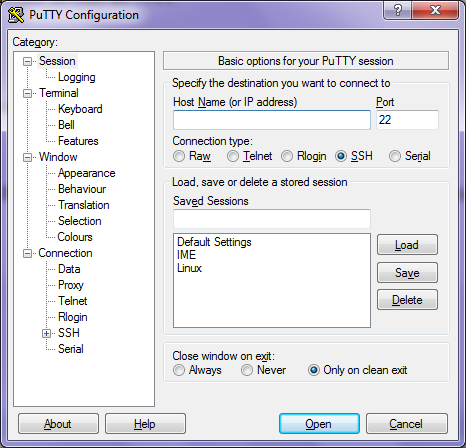
\includegraphics{putty}

\caption{Tela inicial do PuTTY}


\end{figure}



\subsection{OpenSSH Client}

É um programa de terminal. Aqui vai uma lista de exemplos de comandos:
\begin{enumerate}
\item \texttt{ssh destino} ; Conecta-se em destino, usando o mesmo usuário
que o seu atual.
\item \texttt{ssh jose@destino} ; Conecta-se em destino, com o usuário {}``jose''.
\item \texttt{ssh jose@destino -p 22000} ; Conecta-se em destino na port
22000.
\item \texttt{ssh -i chaveprivada destino} ; Conecta-se em destino, usando
\texttt{chaveprivada} como chave privada de autenticação.
\end{enumerate}

\section{Métodos de Autenticação}


\subsection{Senha }

Aparece um prompt onde você digita a senha, que é então transmitida
de maneira segura para o servidor, e que então verifica se a senha
é válida.


\subsection{Chaves}

Chaves são utilizadas para autenticação automática, e são compostas
de duas partes: a pública e a privada.

A chave pública, você deve disponibilizar para os servidores no qual
você deseja autenticar-se, enquanto que a chave privada deve permanecer
apenas no seu cliente.

Uma dos parâmetros para abrir uma conexão SSH é o caminho para o arquivo
de chave privada que deseja usar. O cliente SSH tentará autenticar-se
com o servidor usando essa chave, e obterá sucesso apenas se o servidor
conhecer (e aceitar) a chave pública associada.

\begin{figure}[b]

\includegraphics{privatekey}

\caption{Uma chave, composta pela parte privada e pública.}
\end{figure}


Como a chave em si é utilizada para a autenticação, deve-se tomar
cuidado para impedir acesso indevido à chave. Uma opção de segurança
é criptografar a chave com uma {}``passphrase'' .


\subsubsection{Agente SSH}

Um agente é um programa que possui uma lista de chaves privadas, onde
o seu cliente, no mesmo computador, tem acesso. Como o agente guarda
as chaves de forma descriptografada, não é necessário digitar senhas
ao usar o agente.

É possível encaminhar o agente atravéz da conexão, permitindo utilizar
as mesmas chaves privadas no destino. 

Cuidado: use agentes SSH, em particular se encaminhar-los pela conexão,
apenas se você confia nos administradores da máquina destino, pois
estes podem acessar os arquivos temporários que o agente usa!


\section{Túneis }

Túneis são formas de encapsular e encaminhar conexões arbitrárias
com a conexão SSH.


\subsection{Local -> Remoto}

O seu cliente SSH local escuta conexões numa port TCP de sua máquina,
encaminha atravéz da conexão segura até um servidor SSH, e este encaminha
seus pacotes para o destino, em uma port especificada.

Note que a port local, o destino e a port no destino são especificadas
por você ao abrir a conexão SSH.

\medskip{}


O exemplo abaixo pode ser replicado no OpenSSH Client com o comando
\texttt{ssh user@servidor -L8080:destino:80} . Note que o destino
pode ser fisicamente o próprio servidor SSH.

\begin{figure}[h]
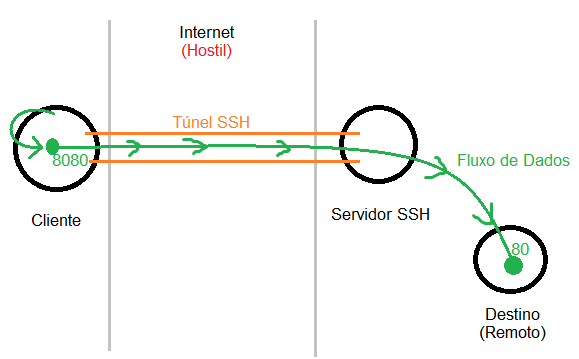
\includegraphics{tunel-local-destino}

\caption{Exemplo de Túnel Local -> Remoto}
\end{figure}


\pagebreak{}


\subsection{Remoto -> Local}

Você configura o servidor SSH para que ele escute uma port específica,
e abre um túnel de conexão segura com ele. O servidor então envia
todo pacote na port escutada para o destino local em uma port específica,
através do seu cliente.

Neste caso também, as ports e o destino são especificados por você,
na criação do túnel.

Em geral, o destino é a própria máquina onde o cliente está sendo
executado.

\medskip{}


O exemplo abaixo pode ser replicado no OpenSSH Client com o comando
\texttt{ssh user@servidor -R8080:destino:80} . Note que o destino
pode ser fisicamente o próprio servidor SSH.

\begin{figure}
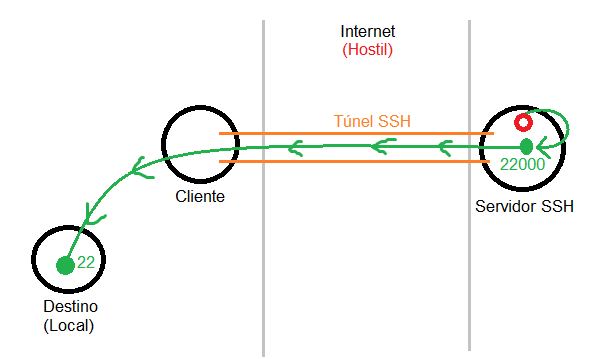
\includegraphics{tunel-destino-local}

\caption{Exemplo de Túnel Remoto -> Local}


\end{figure}



\subsection{Dinâmico}

O seu cliente SSH escuta em uma port especificada em modo de entrada,
podendo também restringí-la a um endereço específico. Sempre que uma
conexão é aberta com essa port, o protocolo da conexão é usado para
decidir o destino final, e a conexão é encaminhada para o servidor
pela conexão segura, que então encaminha por sua vez para o destino.

Isto é útil para criar proxies de maneira segura.


\subsection{X}

O X é um sistema de gerenciador de janelas, que faz distinção entre
servidor (que encapsula o gerenciador de janelas) e clientes (programas
que utilizam e exibem janelas). Isso permite que façamos túneis de
gerenciadores de janelas.

Um túnel X do SSH, é um tipo de {}``display virtual'' na sua sessão
remota, que corresponde a um servidor X na sua máquina local.

Ao abrir um programa remotamente que usa janelas (um cliente X), ele
tentará usar este {}``display virtual'', que é túnel de conexão
segura para seu gerenciador de janelas local.

Assim, você pode usar programas remotamente, ainda aproveitando da
interface gráfica de janelas :P
\end{document}
